\chapter{Технологическая часть}

\section{Средства реализации}

Для программной реализации электронной подписи был выбран язык программирования $Python$. В данном языке есть все требующиеся инструменты для данной лабораторной работы.

\section{Реализация алгоритма}

В листингах~\ref{lst:sign} представлена реализация алгоритма электронной подписи.

\begin{center}
\captionsetup{justification=raggedright,singlelinecheck=off}
\begin{lstlisting}[label=lst:sign,caption=Реализация электронной подписи]
def generate_keys(private_key_path, public_key_path):
    key = RSA.generate(2048)
    private_key = key.export_key()
    public_key = key.publickey().export_key()

    with open(private_key_path, "wb") as f:
        f.write(private_key)
    with open(public_key_path, "wb") as f:
        f.write(public_key)

    print(f"Ключи сгенерированы:\n - Приватный: {private_key_path}\n - Публичный: {public_key_path}")

def sign_file(input_file, private_key_path, signature_file):
    with open(private_key_path, "rb") as f:
        private_key = RSA.import_key(f.read())

    with open(input_file, "rb") as f:
        data = f.read()

    h = SHA256.new(data)
    signature = pkcs1_15.new(private_key).sign(h)

    with open(signature_file, "wb") as f:
        f.write(signature)
    
    print(f"Подпись сохранена в {signature_file}")

def verify_signature(input_file, public_key_path, signature_file):
    with open(public_key_path, "rb") as f:
        public_key = RSA.import_key(f.read())

    with open(input_file, "rb") as f:
        data = f.read()
    with open(signature_file, "rb") as f:
        signature = f.read()

    h = SHA256.new(data)
    try:
        pkcs1_15.new(public_key).verify(h, signature)
        print("Подпись действительна.")
    except (ValueError, TypeError):
        print("Подпись недействительна!")
\end{lstlisting}
\end{center}

\clearpage

\section{Пример работы программы}

На рисунке~\ref{fig:tex} представлен пример работы программы на текстовом фале.

\begin{figure}[h]
    \centering
    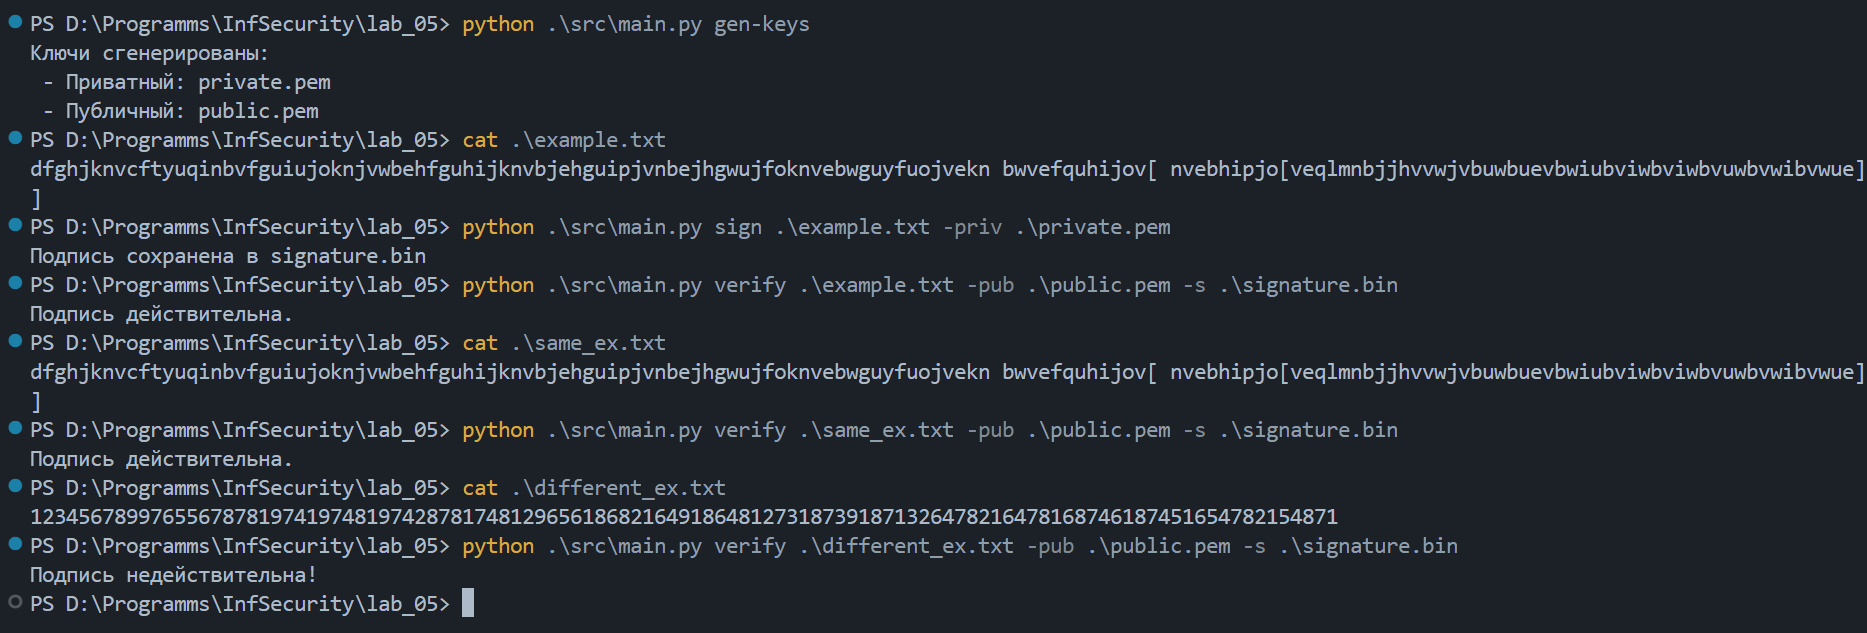
\includegraphics[width=1\linewidth]{images/tex.png}
    \caption{Пример работы программы на текстовом файле}
    \label{fig:tex}
\end{figure}
